\documentclass[aspectratio=169,10pt]{beamer}

\usetheme{Boadilla}
\usecolortheme{beaver}
\usefonttheme{professionalfonts}
\setbeamertemplate{navigation symbols}{}
\setbeamertemplate{footline}[frame number]
\setbeamertemplate{itemize items}[circle]
\setbeamerfont{frametitle}{size=\large,series=\bfseries}
\setbeamercolor{block title}{bg=red!30!black,fg=white}
\setbeamercolor{block body}{bg=red!5}
\setbeamercolor{alertblock title}{bg=orange!80!black,fg=white}
\setbeamercolor{alertblock body}{bg=orange!5}
\setbeamercolor{exampleblock title}{bg=teal!70!black,fg=white}
\setbeamercolor{exampleblock body}{bg=teal!5}

\usepackage{amsmath,amssymb}
\usepackage{booktabs}
\usepackage{tikz}
\usetikzlibrary{arrows.meta,positioning,calc}
\usepackage{xcolor}
\usepackage{array}
\usepackage{colortbl}
\usepackage{microtype}
\usepackage{graphicx}

% Highlight row macro
\newcommand{\best}[1]{\cellcolor{teal!18}\textbf{#1}}

% ─────────────────────────────────────────────────────────────────────────────
\title[Delta Hedging under Stochastic Volatility]{%
  \textbf{Delta Hedging under Stochastic Volatility}\\[0.3em]
  \normalsize When Structure Beats Learning
}
\subtitle{Stochastic Calculus and Its Applications in Finance}
\author{Aditya Nagarsekar, M P Ashish Bhat}
\date{}
% ─────────────────────────────────────────────────────────────────────────────

\begin{document}

% ══════════════════════════════════════════════════════════════════════════════
\begin{frame}
\titlepage
\end{frame}
% ══════════════════════════════════════════════════════════════════════════════

% ──────────────────────────────────────────────────────────────────────────────
\begin{frame}{Outline}
\tableofcontents[hideallsubsections]
\end{frame}
% ──────────────────────────────────────────────────────────────────────────────

% ══════════════════════════════════════════════════════════════════════════════
\section{Problem and Motivation}
% ══════════════════════════════════════════════════════════════════════════════

\begin{frame}{The Delta Hedging Problem}
\begin{columns}[T]
\column{0.52\textwidth}
\textbf{Goal:} Hold a short call; dynamically trade the underlying to offset delta risk.

\medskip
\textbf{BSM textbook solution:} Under frictionless continuous trading,
\[
  \Delta^\star = \Phi(d_1),\quad
  d_1 = \frac{\ln(S/K)+(r+\tfrac{1}{2}\sigma^2)\tau}{\sigma\sqrt{\tau}}
\]
replicates the option perfectly.

\medskip
\textbf{But practice violates two key assumptions:}
\begin{enumerate}
  \item Trading is \emph{discrete} and \emph{costly} — proportional TC $\kappa|\Delta\delta|\cdot S$
  \item Volatility is \emph{unknown} and \emph{stochastic}
\end{enumerate}

\column{0.44\textwidth}
\begin{block}{Research Questions}
\begin{itemize}
  \item Can RL learn a better hedge than BSM?
  \item Does an LSTM vol forecast improve hedging?
  \item How do they combine?
\end{itemize}
\end{block}

\vspace{0.5em}
\begin{exampleblock}{Setting}
Nifty~50 options, 2010--2024\\
51 non-overlapping 21-day test windows\\
Transaction cost $\kappa = 0.001$
\end{exampleblock}
\end{columns}
\end{frame}

% ──────────────────────────────────────────────────────────────────────────────
\begin{frame}{Mathematical Framework: Risk-Neutral Pricing}
Under the physical measure $\mathbb{P}$, the stock follows GBM:
\[
  dS_t = \mu S_t\,dt + \sigma S_t\,dW_t^{\mathbb{P}}
\]
\textbf{Girsanov's theorem} (change of measure):
\[
  \frac{d\mathbb{Q}}{d\mathbb{P}}\bigg|_{\mathcal{F}_T}
  = \exp\!\Bigl(-\theta W_T^{\mathbb{P}} - \tfrac{1}{2}\theta^2 T\Bigr),
  \quad \theta = \frac{\mu - r}{\sigma}
\]
Under $\mathbb{Q}$, the discounted stock $e^{-rt}S_t$ is a \emph{martingale}, and the fair option price is:
\[
  V_0 = e^{-rT}\,\mathbb{E}^{\mathbb{Q}}\!\left[(S_T - K)^+\right]
\]
\begin{columns}[T]
\column{0.48\textwidth}
\begin{block}{BSM PDE (Itô's Lemma + No-Arbitrage)}
\[
  \frac{\partial V}{\partial t} + \frac{1}{2}\sigma^2 S^2 \frac{\partial^2 V}{\partial S^2}
  + rS\frac{\partial V}{\partial S} - rV = 0
\]
\end{block}
\column{0.48\textwidth}
\begin{block}{CRR Binomial Tree}
$u = e^{\sigma\sqrt{\Delta t}}$,\quad $d = 1/u$
\[
  p = \frac{e^{r\Delta t}-d}{u-d}, \quad N=100
\]
Converges to BSM as $N\to\infty$
\end{block}
\end{columns}
\end{frame}

% ──────────────────────────────────────────────────────────────────────────────
\begin{frame}{Hedging Error Decomposition}
Under discrete rebalancing, the one-step hedging error can be decomposed:
\[
  \varepsilon_t = \underbrace{(\delta_t - \Delta_t^\star)\,\Delta S_t}_{\text{controllable: hedge gap}}
               - \underbrace{\tfrac{1}{2}\Gamma\left[(\Delta S_t)^2 - \sigma^2 S_t^2 \Delta t\right]}_{\text{irreducible: gamma noise}}
\]

\begin{columns}[T]
\column{0.48\textwidth}
\begin{alertblock}{Controllable term}
How far is implemented hedge $\delta_t$ from analytic target $\Delta_t^\star$?\\[0.3em]
\textbf{Lever 1:} Better $\sigma$ estimate $\Rightarrow$ better $\Delta^\star$\\
\textbf{Lever 2:} Better execution rule
\end{alertblock}

\column{0.48\textwidth}
\begin{block}{Gamma noise variance}
\[
  \mathrm{Var}(\text{gamma noise}) = \tfrac{1}{2}\sigma^4 S^4 \Gamma^2 (\Delta t)^2
\]
Peaks ATM near expiry; expectation $= 0$ by Itô's isometry.\\
\emph{Irreducible with daily rebalancing.}
\end{block}
\end{columns}

\medskip
\textbf{Implication:} RL must beat BSM on the \emph{controllable} term — a hard task when BSM's $\Phi(d_1)$ is already analytically optimal under GBM.
\end{frame}

% ══════════════════════════════════════════════════════════════════════════════
\section{Project Overview}
% ══════════════════════════════════════════════════════════════════════════════

\begin{frame}{Project Architecture}
\centering
\resizebox{0.55\textwidth}{!}{%
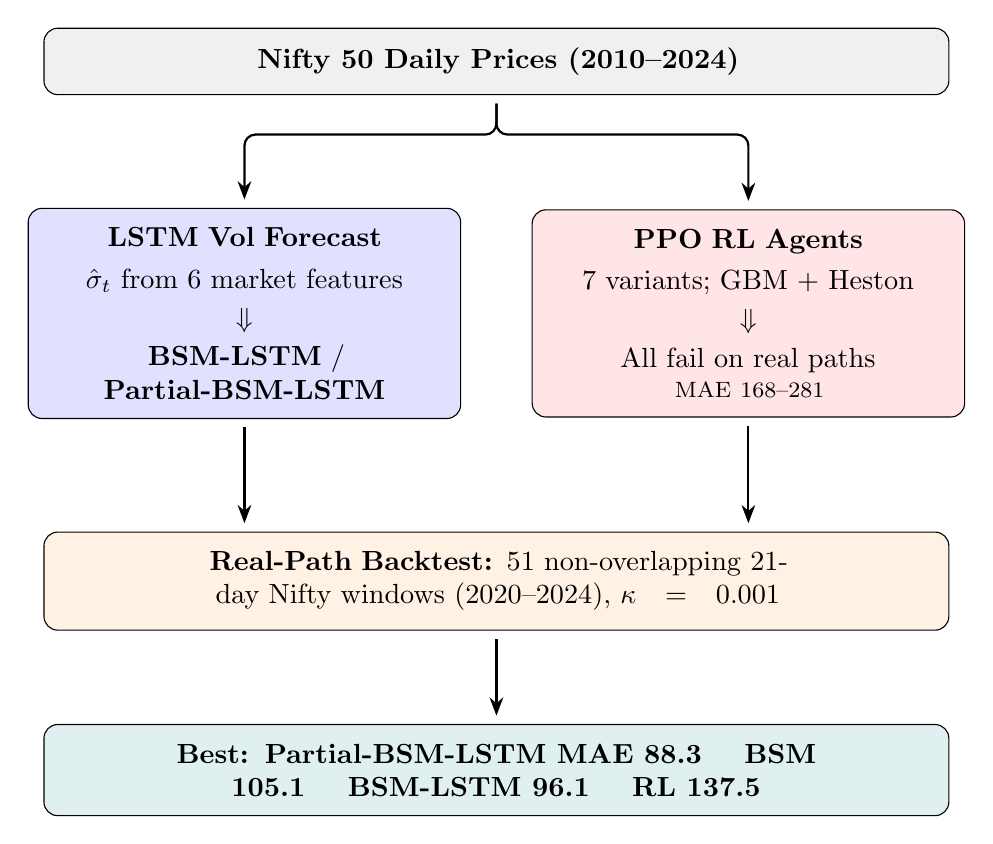
\begin{tikzpicture}[
  arr/.style={-Stealth, thick, rounded corners=4pt, shorten >=3pt, shorten <=3pt},
  tbox/.style={draw, rounded corners=5pt, fill=gray!12, text width=11cm,
               align=center, font=\normalsize\bfseries, inner sep=7pt},
  lbox/.style={draw, rounded corners=5pt, fill=blue!12, text width=5.0cm,
               align=center, font=\normalsize, inner sep=7pt},
  rbox/.style={draw, rounded corners=5pt, fill=red!10, text width=5.0cm,
               align=center, font=\normalsize, inner sep=7pt},
  bbox/.style={draw, rounded corners=5pt, fill=orange!10, text width=11cm,
               align=center, font=\normalsize, inner sep=7pt},
  resbox/.style={draw, rounded corners=5pt, fill=teal!12, text width=11cm,
                 align=center, font=\normalsize\bfseries, inner sep=7pt},
]
\node[tbox] (data) at (0,0)
  {Nifty~50 Daily Prices (2010--2024)};

\node[lbox] (left) at (-3.2,-3.2)
  {\textbf{LSTM Vol Forecast}\\[3pt]
   $\hat\sigma_t$ from 6 market features\\[2pt]
   $\Downarrow$\\[2pt]
   \textbf{BSM-LSTM} / \textbf{Partial-BSM-LSTM}};

\node[rbox] (right) at (3.2,-3.2)
  {\textbf{PPO RL Agents}\\[3pt]
   7 variants; GBM + Heston\\[2pt]
   $\Downarrow$\\[2pt]
   All fail on real paths\\[-1pt]
   {\footnotesize MAE 168--281}};

\node[bbox] (bt) at (0,-6.6)
  {\textbf{Real-Path Backtest:} 51 non-overlapping 21-day Nifty windows (2020--2024), $\kappa=0.001$};

\node[resbox] (res) at (0,-9.0)
  {Best: \textbf{Partial-BSM-LSTM} MAE \textbf{88.3} \quad
   BSM 105.1 \quad BSM-LSTM 96.1 \quad RL 137.5};

\draw[arr] (data.south) -- ++(0,-0.5) -| (left.north);
\draw[arr] (data.south) -- ++(0,-0.5) -| (right.north);
\draw[arr] (left.south)  -- (left.south  |- bt.north);
\draw[arr] (right.south) -- (right.south |- bt.north);
\draw[arr] (bt.south)    -- (res.north);
\end{tikzpicture}}
\end{frame}

% ══════════════════════════════════════════════════════════════════════════════
\section{Component 1: RL for Hedging}
% ══════════════════════════════════════════════════════════════════════════════

\begin{frame}{PPO Agent: Setup}
\begin{columns}[T]
\column{0.52\textwidth}
\textbf{Environment:} Simulated GBM (and Heston) paths for a 21-day European call

\medskip
\textbf{State (base):} $s_t = \bigl(\text{moneyness},\; \tau/T,\; \delta_{t-1}\bigr)$; extended variants additionally include $\hat\sigma_t$ and BSM-$\Delta$ depending on the variant

\medskip
\textbf{Action:} $a_t = \delta_t \in [0,1]$

\medskip
\textbf{Reward (base):}
\[
  r_t = -\varepsilon_t^2 - \kappa|\delta_t - \delta_{t-1}|S_t
\]
Penalises squared one-step hedging error plus proportional TC

\smallskip
Itô-inspired variants subtract the gamma noise term; other variants add $\Gamma$ as a state feature — explored across the 6 extensions

\column{0.44\textwidth}
\begin{block}{PPO Clipping}
\[
  L^{\text{CLIP}} = \mathbb{E}\!\left[\min\!\left(r_t A_t,\;\mathrm{clip}(r_t,1\pm\epsilon)A_t\right)\right]
\]
Conservative updates prevent destructive policy changes in noisy financial rewards
\end{block}

\medskip
\begin{exampleblock}{6 Variants Tested}
\begin{itemize}\itemsep0pt
  \item Domain randomisation ($\sigma \sim U[0.10,0.40]$)
  \item LSTM-conditioned PPO
  \item Anchor-controller (adjust around BSM $\Delta$)
  \item Discrete DQN
  \item Heston environment
  \item Reward design variants
\end{itemize}
\end{exampleblock}
\end{columns}
\end{frame}

% ──────────────────────────────────────────────────────────────────────────────
\begin{frame}{RL Results in Simulation}
\begin{columns}[T]
\column{0.55\textwidth}
\begin{center}
\small
\begin{tabular}{lcc}
\toprule
Agent (variant) & MAE & BSM-$\Delta$ Corr. \\
\midrule
BSM (analytic) & \best{0.284} & --- \\
A: GBM + MSE (base) & 0.830 & 0.946 \\
B: GBM + It\^{o} reward & 0.926 & 0.935 \\
C: Heston + MSE & 0.790 & 0.963 \\
D: Heston + It\^{o} & 0.790 & 0.958 \\
E: GBM + It\^{o} + $\Gamma$ obs & 0.764 & 0.957 \\
F: GBM + domain rand.\ $\sigma$ & \best{0.723} & \textbf{0.964} \\
\bottomrule
\end{tabular}
\end{center}

\medskip
\textbf{Natural habitat} (varying-$\sigma$ env, fair comparison):
\begin{itemize}\itemsep1pt
  \item LSTM-RL MAE: \textbf{0.407} vs 1.435 constant-$\sigma$ baseline
  \item \textbf{$-72\%$ MAE}, \textbf{$-64\%$ CVaR$_{95}$} ($p < 0.001$, paired bootstrap)
  \item CVaR: $-1.85$ vs $-5.08$ — catastrophic tails eliminated
\end{itemize}

\column{0.42\textwidth}
\begin{exampleblock}{LSTM-guided BSM still wins}
Even in the natural habitat, BSM-LSTM (MAE 0.227) outperforms LSTM-RL (0.407). The analytic formula re-evaluates $\Phi(d_1)$ at every step exactly; RL generalises from training imperfectly.
\end{exampleblock}

\medskip
\begin{block}{Utility dominance ($J_\lambda = \text{MAE} + \lambda\cdot\text{TC}$)}
LSTM-guided BSM wins at \emph{every} risk-aversion $\lambda$:\\
$J_1$: \textbf{0.339} vs BSM 0.430 vs RL 0.895\\
$J_5$: \textbf{0.786} vs BSM 1.015 vs RL 1.424
\end{block}
\end{columns}
\end{frame}

% ══════════════════════════════════════════════════════════════════════════════
\section{Component 2: LSTM Volatility Forecasting}
% ══════════════════════════════════════════════════════════════════════════════

\begin{frame}{Volatility Forecasting: Why It Matters}
\textbf{The Vega link:} A $1\%$-point error in $\sigma$ propagates to a pricing error of
\[
  \text{price error} \approx \text{Vega} \times 0.01 = S\sqrt{\tau}\,\phi(d_1) \times 0.01
\]
For ATM Nifty options ($S\!\approx\!22{,}000$, $\tau=21/252$): $\approx$ \textbf{25 points per 1 percentage-point vol error} (typical 13--18 pp forecasting error $\Rightarrow$ 330--450 points total pricing impact).

\medskip
\begin{columns}[T]
\column{0.48\textwidth}
\begin{block}{LSTM Architecture}
\begin{itemize}\itemsep2pt
  \item 2-layer stacked LSTM, hidden dims \textbf{64 + 32}
  \item Sequence length: \textbf{60 trading days}
  \item 5 features: rv5, rv21, log-return, momentum, rv\_ratio
  \item Target: $\sigma_{\text{realized}}$ over next 21 days
  \item Train 70\% / Val 15\% / Test 15\% (chronological)
\end{itemize}
\end{block}

\column{0.48\textwidth}
\begin{block}{Key Feature: rv\_ratio}
\[
  \text{rv\_ratio} = \frac{\text{rv5}}{\text{rv21}}
\]
Encodes whether short-horizon vol is elevated vs.\ medium-horizon — a regime-change signal GARCH has no equivalent for.
\end{block}
\end{columns}
\end{frame}

% ──────────────────────────────────────────────────────────────────────────────
\begin{frame}{Volatility Forecasting Results}
\begin{columns}[T]
\column{0.52\textwidth}
\begin{center}
\small
\begin{tabular}{lccc}
\toprule
Model & RMSE & MAE & Dir. Acc. \\
\midrule
\best{LSTM} & \best{0.0203} & \best{0.0114} & 0.503 \\
GARCH(1,1) & 0.0254 & 0.0194 & 0.479 \\
rv21 naive & \cellcolor{orange!15}\textbf{0.0102} & \cellcolor{orange!15}\textbf{0.0043} & \cellcolor{orange!15}\textbf{0.544} \\
India VIX & 0.0453 & 0.0344 & 0.523 \\
\bottomrule
\end{tabular}
\end{center}
\vspace{0.5em}
\begin{exampleblock}{LSTM vs GARCH}
\textbf{41\% lower MAE} (0.0114 vs 0.0194)\\
\textbf{20\% lower RMSE} (0.0203 vs 0.0254)
\end{exampleblock}

\column{0.44\textwidth}
\begin{alertblock}{The rv21 paradox}
A \emph{naive persistence baseline} beats all models at the 21-day horizon.\\[0.4em]
\textbf{Why?} The trailing window $[t\!-\!20,t]$ overlaps \textbf{86\%} with the forward target $[t\!+\!1,t\!+\!21]$ under strong volatility clustering (Nifty Hurst exponent $\approx 0.65$), giving rv21 an inherent informational advantage. Any more complex model must improve on something already near-optimal. 
rv21 is a \emph{transparency control}, not a model to beat.
\end{alertblock}
\begin{block}{Directional accuracy $\approx 50\%$}
Persistence (predicts same direction) and mean-reversion (predicts opposite) cancel. Level prediction is the right metric.
\end{block}
\end{columns}
\end{frame}

% ──────────────────────────────────────────────────────────────────────────────
\begin{frame}{India VIX and the Variance Risk Premium}
\begin{columns}[T]
\column{0.55\textwidth}
\textbf{Why does India VIX underperform?}

\medskip
India VIX is implied volatility — it is computed under the risk-neutral measure $\mathbb{Q}$:
\[
  \sigma_{\text{VIX}}^2 = \mathbb{E}^{\mathbb{Q}}\!\left[\int_0^T \sigma_t^2\,dt\right] + \text{VRP}
\]
The \textbf{Volatility Risk Premium} (VRP $\approx 4$--$6\%$ annualised) represents what investors pay for variance protection — a systematic upward bias of 4--6\% over realised vol.

\medskip
LSTM forecasts under $\mathbb{P}$ (physical measure); using VIX directly as a forecast overstates realised vol.

\column{0.41\textwidth}
\begin{alertblock}{Girsanov in action}
The market price of vol risk $\theta_v$ shifts $\mathbb{Q}$ away from $\mathbb{P}$:
\[
  \sigma_{\text{impl}} \approx \sigma_{\text{realised}} + \text{VRP}
\]
Using implied vol without VRP correction is a \emph{measure mismatch}.
\end{alertblock}

\medskip
\begin{block}{Practical implication}
India VIX would need a data-driven VRP correction before it can be used as a vol forecast for physical-measure hedging.
\end{block}
\end{columns}
\end{frame}

% ══════════════════════════════════════════════════════════════════════════════
\section{Integration: Option Pricing \& Backtesting}
% ══════════════════════════════════════════════════════════════════════════════

\begin{frame}{Option Pricing Horse-Race}
\begin{columns}[T]
\column{0.50\textwidth}
\textbf{Overall MAE} (ATM synthetic, $T=21/252$):
\begin{center}
\small
\begin{tabular}{lcc}
\toprule
Method & MAE & Note \\
\midrule
GARCH(1,1)        & 43.6 & Over-reacts to spikes \\
LSTM              & 30.3 & rv21 dominates at 21d \\
\best{Historical (rv21)} & \best{18.6} & Persistence effect \\
\best{Implied (lagged)} & \best{18.7} & Freshest market info \\
\bottomrule
\end{tabular}
\end{center}

\medskip\small
\textbf{By moneyness} (MAE, implied best everywhere):
\begin{center}
\begin{tabular}{lccc}
\toprule
 & OTM & ATM & ITM \\
\midrule
Historical & 9.56 & 17.67 & 7.70 \\
\best{Implied} & \best{8.56} & \best{17.31} & \best{6.80} \\
LSTM & 14.27 & 25.88 & 11.37 \\
\bottomrule
\end{tabular}
\end{center}

\column{0.55\textwidth}
\begin{block}{Why rv21 $\approx$ implied in pricing}
Both are slow-moving, high-overlap proxies for the next 21-day vol. The 86\% window overlap makes trailing rv21 nearly as informative as yesterday's IV.
\end{block}
\begin{alertblock}{Why LSTM lags in pricing}
At the 21-day horizon, rv21 persistence dominates. LSTM's advantage is in longer-horizon \emph{regime} shifts; at this lag it adds less than persistence alone.\\[0.3em]
LSTM still beats GARCH by \textbf{31\%} (30.3 vs 43.6).
\end{alertblock}
\begin{exampleblock}{Why LSTM still matters for hedging}
Pricing uses fixed-point vol; hedging uses it \emph{pathwise} — LSTM corrects local $\sigma$ deviations step-by-step via the Vega link.
\end{exampleblock}
\end{columns}
\end{frame}

% ──────────────────────────────────────────────────────────────────────────────
\begin{frame}{Real-Path Hedging Backtest}
\textbf{Setup:} 51 non-overlapping 21-day windows on Nifty~50 (2020--2024), $\kappa=0.001$

\begin{center}
\small
\begin{tabular}{lcccc}
\toprule
Strategy & Mean P\&L & Std P\&L & MAE [95\% CI] & Mean TC \\
\midrule
BSM daily (rv21)         & $+$1.19   & 162.2 & 105.1\ [74.7,\;141.0] & 36.0 \\
RL PPO (rv21)            & $-$13.4   & 205.0 & 137.5\ [99.3,\;181.1] & 39.4 \\
BSM-LSTM                 & $+$7.48   & 144.0 & 96.1\ \ [69.6,\;127.2] & 35.6 \\
\best{Partial-BSM-LSTM}  & \best{$+$1.02} & \best{134.6} & \best{88.3\ [63.6,\;118.4]} & \best{27.4} \\
\bottomrule
\end{tabular}
\end{center}

\vspace{0.4em}
\begin{columns}[T]
\column{0.32\textwidth}
\begin{exampleblock}{Best model wins}
Partial-BSM-LSTM vs BSM:
\begin{itemize}
  \item MAE: $105.1 \to \mathbf{88.3}$ \;(\textbf{$-16\%$})
  \item TC: $36.0 \to \mathbf{27.4}$ \;(\textbf{$-24\%$})
\end{itemize}
\medskip
\textbf{Tail risk:} BSM CVaR$_{95}$ $= -457$ vs RL $= -535$\\
RL has \textbf{17\% heavier tails} on real paths
\end{exampleblock}

\column{0.64\textwidth}
\begin{alertblock}{Statistical caveat}
BSM-LSTM vs Partial-BSM-LSTM: $p=0.121$ (not significant at 51 windows).
BSM vs RL: $p=0.013$ — significant.
\end{alertblock}

\begin{block}{High-vol regime ($\sigma>25\%$)}
\begin{tabular}{lcc}
\small Regime & BSM & RL \\
\midrule
\small Low ($<$15\%) & 95.6 & 117.9 \\
\small Med (15--25\%) & 88.2 & 154.8 \\
\small High ($>$25\%) & 384.5 & \textbf{377.7} \\
\end{tabular}
{\footnotesize high-vol domain randomisation helps}
\end{block}
\end{columns}
\end{frame}

% ══════════════════════════════════════════════════════════════════════════════
\section{RL Failure Analysis}
% ══════════════════════════════════════════════════════════════════════════════

\begin{frame}{Why RL Fails on Real Paths}
\begin{columns}[T]
\column{0.52\textwidth}
\textbf{All pure-RL variants fail to outperform BSM:}

\begin{center}
\small
\begin{tabular}{lc}
\toprule
RL Variant & Real-path MAE \\
\midrule
Base PPO (rv21)            & 137.5 \\
LSTM-conditioned PPO       & 168.2 \\
Anchor-residual (LSTM)     & 214.9 \\
DQN discrete (LSTM)        & 251.8 \\
Anchor-fraction (DR/LSTM)  & 281.1 \\
\midrule
\textit{BSM baseline}      & \textit{105.1} \\
\textit{Hybrid BSM+DR-RL}  & \textit{100.0} \\
\bottomrule
\end{tabular}
\end{center}
\vspace{-2pt}
{\footnotesize\textit{Hybrid shows promise but still beaten by Partial-BSM-LSTM (88.3)}}

\column{0.44\textwidth}
\begin{alertblock}{Failure mode: underhedging}
Policies converge to \textbf{low-turnover underhedging}: reduce trading costs but allow large residual hedge error.\\[0.2em]
TC lower (39.4 vs 36.0) — policy learned to \emph{trade less}, not hedge better.\\[0.2em]
\textbf{Tail risk:} RL CVaR$_{95}$ $= -535$ vs BSM $-457$ — RL has \textbf{17\% heavier real-path tails}.
\end{alertblock}
\begin{block}{Root cause: distribution shift}
GBM training lacks real Nifty's volatility clustering, heavy tails, and regime changes.\\[0.2em]
\textbf{Exception:} in the high-vol regime ($\sigma\!>\!25\%$), domain-randomised RL (MAE 377.7) marginally beats BSM (384.5) — the only real-path RL win.
\end{block}
\end{columns}
\end{frame}

% ──────────────────────────────────────────────────────────────────────────────
\begin{frame}{The Itô Reward Paradox}
\begin{columns}[T]
\column{0.55\textwidth}
\textbf{Base (A): squared hedging error}
\[
  r_t^A = -\varepsilon_t^2 - \kappa|\delta_t - \delta_{t-1}|S_t
\]
\textbf{Variant B: subtract gamma noise from reward}
\[
  r_t^B = -\!\left(\varepsilon_t - \tfrac{1}{2}\Gamma\bigl[(\Delta S_t)^2 - \sigma^2 S_t^2\Delta t\bigr]\right)^{\!2} - \kappa|\delta_t - \delta_{t-1}|S_t
\]
In theory, removes irreducible noise to sharpen the signal.\\[0.3em]
\textbf{In practice, B is \emph{worse} than A} (MAE $0.926$ vs $0.830$).

\medskip
\textbf{Problem:} Near convergence ($\delta_t\to\Delta^\star_t$) the gamma term vanishes — so does the gradient, removing the reinforcement signal.

\medskip
\textbf{Variant E:} adds $\Gamma$ as a \emph{state observation} instead. Gradient preserved; achieves MAE $0.764$ — best among all variants without domain randomisation.

\column{0.41\textwidth}
\begin{alertblock}{Why structure helps RL}
Providing the gamma observation gives the agent structural guidance about curvature risk — information that pure reward shaping obscures.\\[0.4em]
Even with this, RL still fails to beat BSM on real paths.
\end{alertblock}

\medskip
\begin{exampleblock}{Lesson}
RL in finance is fragile to reward design. The Itô decomposition is mathematically elegant but doesn't straightforwardly translate to a better reward function.
\end{exampleblock}
\end{columns}
\end{frame}

% ══════════════════════════════════════════════════════════════════════════════
\section{Partial-BSM-LSTM: The Winning Approach}
% ══════════════════════════════════════════════════════════════════════════════

\begin{frame}{Partial-BSM-LSTM: Design and Intuition}
\begin{columns}[T]
\column{0.52\textwidth}
\textbf{Executed hedge at time $t$:}
\[
  \delta_t =
  \begin{cases}
    \delta_{t-1}, & |\Delta_t^\star - \delta_{t-1}| \le \theta \\[4pt]
    \delta_{t-1} + \alpha(\Delta_t^\star - \delta_{t-1}), & \text{otherwise}
  \end{cases}
\]
where $\Delta_t^\star = \Phi(d_1)$ computed at LSTM forecast $\hat\sigma_t$.

\medskip
Best hyperparameters: $\alpha = 0.9$, $\theta = 0.1$

\medskip
\textbf{Intuition from the decomposition:}
\begin{itemize}
  \item Small adjustments ($|\Delta^\star - \delta| \le \theta$) are dominated by TC + gamma noise $\Rightarrow$ hold
  \item Large deviations require correction $\Rightarrow$ partial step
  \item $\alpha < 1$ smooths the hedge path, further reducing TC
\end{itemize}

\column{0.44\textwidth}
\begin{block}{Why this beats full rebalancing}
Full rebalancing (BSM-LSTM, $\alpha=1$, $\theta=0$) achieves MAE 96.1 but TC 35.6.\\[0.3em]
Partial rule: MAE \textbf{88.3}, TC \textbf{27.4}.\\[0.3em]
Reduced TC leaves more capital to absorb genuine hedging error.
\end{block}

\medskip
\begin{exampleblock}{vs.\ RL anchor-controller}
RL also tried partial execution around a BSM anchor — but converged to a degenerate low-trading policy.\\[0.3em]
The key difference: \emph{deterministic} partial rebalancing is transparent and doesn't overfit to simulation.
\end{exampleblock}
\end{columns}
\end{frame}

% ──────────────────────────────────────────────────────────────────────────────
\begin{frame}{Performance at a Glance}
% Bar widths: MAE * (7.50cm / 281.1)  scale = 0.02668 cm per unit
% 88.3->2.36  96.1->2.56  100.0->2.67  105.1->2.80
% 137.5->3.67  214.9->5.73  281.1->7.50
\begin{center}
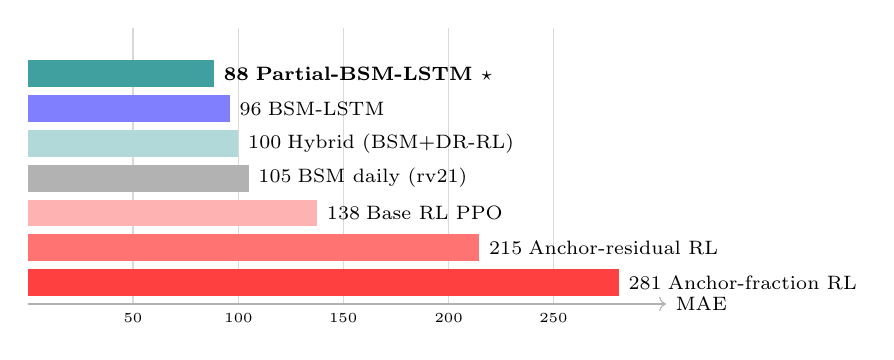
\begin{tikzpicture}[y=0.68cm, x=1cm]
  % grid lines at MAE = 50,100,150,200,250
  \foreach \gx/\lbl in {1.33/50, 2.67/100, 4.00/150, 5.34/200, 6.67/250}{
    \draw[gray!30,thin] (\gx,-0.15) -- (\gx,5.0);
    \node[below,font=\tiny] at (\gx,-0.15) {\lbl};
  }
  \draw[->,thin,gray!60] (0,-0.15) -- (8.1,-0.15) node[right,font=\scriptsize,black] {MAE};
  % bars: bottom=best, top=worst; height 0.50, gap 0.15
  \fill[teal!75]   (0,3.90) rectangle (2.36,4.40);
  \node[right,font=\scriptsize\bfseries] at (2.36,4.15) {\textbf{88}\;Partial-BSM-LSTM $\star$};
  \fill[blue!50]   (0,3.25) rectangle (2.56,3.75);
  \node[right,font=\scriptsize] at (2.56,3.50) {96\;BSM-LSTM};
  \fill[teal!30]   (0,2.60) rectangle (2.67,3.10);
  \node[right,font=\scriptsize] at (2.67,2.85) {100\;Hybrid (BSM+DR-RL)};
  \fill[gray!60]   (0,1.95) rectangle (2.80,2.45);
  \node[right,font=\scriptsize] at (2.80,2.20) {105\;BSM daily (rv21)};
  \fill[red!30]    (0,1.30) rectangle (3.67,1.80);
  \node[right,font=\scriptsize] at (3.67,1.55) {138\;Base RL PPO};
  \fill[red!55]    (0,0.65) rectangle (5.73,1.15);
  \node[right,font=\scriptsize] at (5.73,0.90) {215\;Anchor-residual RL};
  \fill[red!75]    (0,0.00) rectangle (7.50,0.50);
  \node[right,font=\scriptsize] at (7.50,0.25) {281\;Anchor-fraction RL};
\end{tikzpicture}
\end{center}

\begin{columns}[T]
\column{0.5\textwidth}
\begin{exampleblock}{LSTM + execution gains}
\textbf{LSTM vol input}: $105 \to 96$ ($-8.6\%$)\\
\textbf{Partial execution}: $96 \to 88$ ($-8.1\%$)\\
\textbf{Combined gain}: $105 \to \mathbf{88}$ (\textbf{$-16\%$})
\end{exampleblock}

\column{0.46\textwidth}
\begin{alertblock}{RL outcome}
Most RL variants sit well above BSM; the hybrid (100) shows some promise but is still beaten by the deterministic partial rule (88).
\end{alertblock}
\end{columns}
\end{frame}

% ══════════════════════════════════════════════════════════════════════════════
\section{Discussion and Conclusions}
% ══════════════════════════════════════════════════════════════════════════════

\begin{frame}{Four Key Lessons}
\begin{enumerate}
\setlength\itemsep{0.9em}

  \item \textbf{Volatility estimation dominates performance.}\\
  BSM is already strong; improving $\sigma$ from rv21 to LSTM produces a more reliable gain than replacing the hedge rule. Vega amplifies every vol forecasting improvement.

  \item \textbf{Execution strategy matters more than learning delta directly.}\\
  Partial-BSM-LSTM outperforms full BSM-LSTM \emph{not} by changing the hedge target, but by changing how aggressively the portfolio is moved toward it.

  \item \textbf{RL struggles because of noise and distribution shift.}\\
  Policies trained under GBM do not transfer to real Nifty dynamics (clustering, heavy tails, regimes). More expressive simulation (Heston) helps slightly in-simulation but anchor-based RL variants fail even more severely on real paths.

  \item \textbf{Simple deterministic control around a strong analytic baseline beats RL.}\\
  The best model in the study combines analytic structure, learned vol, and a transparent partial-adjustment rule. No end-to-end learning required.

\end{enumerate}
\end{frame}

% ──────────────────────────────────────────────────────────────────────────────
\begin{frame}{Conclusion}
\begin{columns}[T]
\column{0.55\textwidth}
\textbf{Bottom line:}

\begin{center}
\Large
\textbf{Structure + Good Inputs + Simple Control}\\[0.3em]
$\succ$\\[0.3em]
\textbf{Complex End-to-End Learning}
\end{center}
BSM remains a very strong baseline. It can be improved:
\begin{itemize}
  \item \textbf{Better inputs:} LSTM $-41\%$ MAE over GARCH; wins $J_\lambda$ at every $\lambda$
  \item \textbf{Better execution:} Partial rule $-24\%$ TC, $-16\%$ MAE
  \item \textbf{Distributional alignment:} LSTM-RL $-72\%$ MAE and $-64\%$ CVaR$_{95}$ in natural habitat ($p<0.001$)
  \item \textbf{Tail safety:} BSM CVaR $-457$ vs RL $-535$ on real paths
\end{itemize}

\column{0.41\textwidth}
\begin{block}{Future Directions}
\begin{itemize}\itemsep4pt
  \item \textbf{Richer simulation:} jump-diffusion, regime-switching GBM
  \item \textbf{VRP correction:} adjust LSTM forecasts toward $\mathbb{Q}$ measure
  \item \textbf{Longer test windows:} $n\gg51$ for statistical significance of partial rebalancing gain
  \item \textbf{Model-based RL:} learn vol model directly from data, then plan
\end{itemize}
\end{block}
\end{columns}
\end{frame}

% ──────────────────────────────────────────────────────────────────────────────
\begin{frame}{References}
\small
\begin{itemize}\itemsep3pt
  \item F.~Black and M.~Scholes, ``The pricing of options and corporate liabilities,'' \textit{J. Political Economy}, 1973.
  \item R.~C.~Merton, ``Theory of rational option pricing,'' \textit{Bell J. Economics}, 1973.
  \item J.~C.~Cox, S.~A.~Ross, M.~Rubinstein, ``Option pricing: A simplified approach,'' \textit{J. Financial Economics}, 1979.
  \item S.~L.~Heston, ``A closed-form solution for options with stochastic volatility,'' \textit{Rev. Financial Studies}, 1993.
  \item T.~Bollerslev, ``Generalised autoregressive conditional heteroskedasticity,'' \textit{J. Econometrics}, 1986.
  \item S.~Hochreiter and J.~Schmidhuber, ``Long short-term memory,'' \textit{Neural Computation}, 1997.
  \item J.~Schulman et al., ``Proximal policy optimization algorithms,'' \textit{arXiv:1707.06347}, 2017.
  \item H.~Buehler et al., ``Deep hedging,'' \textit{Quantitative Finance}, 2019.
  \item S.~E.~Shreve, \textit{Stochastic Calculus for Finance II}, Springer, 2004.
\end{itemize}
\end{frame}

% ──────────────────────────────────────────────────────────────────────────────
\begin{frame}[plain]
\begin{center}
\vspace{1.5cm}
{\LARGE \textbf{Thank You}}

\vspace{1.5cm}
{\large Delta Hedging under Stochastic Volatility:\\[0.3em]
When Structure Beats Learning}

\vspace{1cm}

\begin{tikzpicture}
  \draw[teal!70!black, very thick, rounded corners=8pt]
    (-5,-0.7) rectangle (5,0.7);
  \node[font=\large] at (0,0) {%
    Partial-BSM-LSTM:\quad MAE $\mathbf{88.3}$\quad TC $\mathbf{27.4}$\quad
    \textcolor{teal!70!black}{Best result}};
\end{tikzpicture}

\vspace{1cm}
\textit{Aditya Nagarsekar}
\end{center}
\end{frame}
% ══════════════════════════════════════════════════════════════════════════════

\end{document}